\documentclass[../TDE7_ocrsf.tex]{subfiles}%

\begin{document}
\section[s]"3"{Système à deux ressorts}
\enonce{%
	\noindent
	\begin{minipage}{0.60\linewidth}
		Un point matériel $M$, de masse $m$, peut se déplacer sur une tige
		\emph{horizontale} parallèle à l'axe $Ox$ au sein d'un fluide visqueux qui
		exerce sur lui la force de frottement $\vec{f} = - h\vec{v}$ avec
		$\vec{v}$ le vecteur vitesse de $M$ dans le référentiel galiléen
		$\mathcal{R}$ du laboratoire. Les frottements entre $M$ et l'axe
		horizontal sont négligeables. On repère $M$ par son abscisse $x(t)$.
	\end{minipage}
	\hfill
	\begin{minipage}{0.35\linewidth}
		\begin{center}
			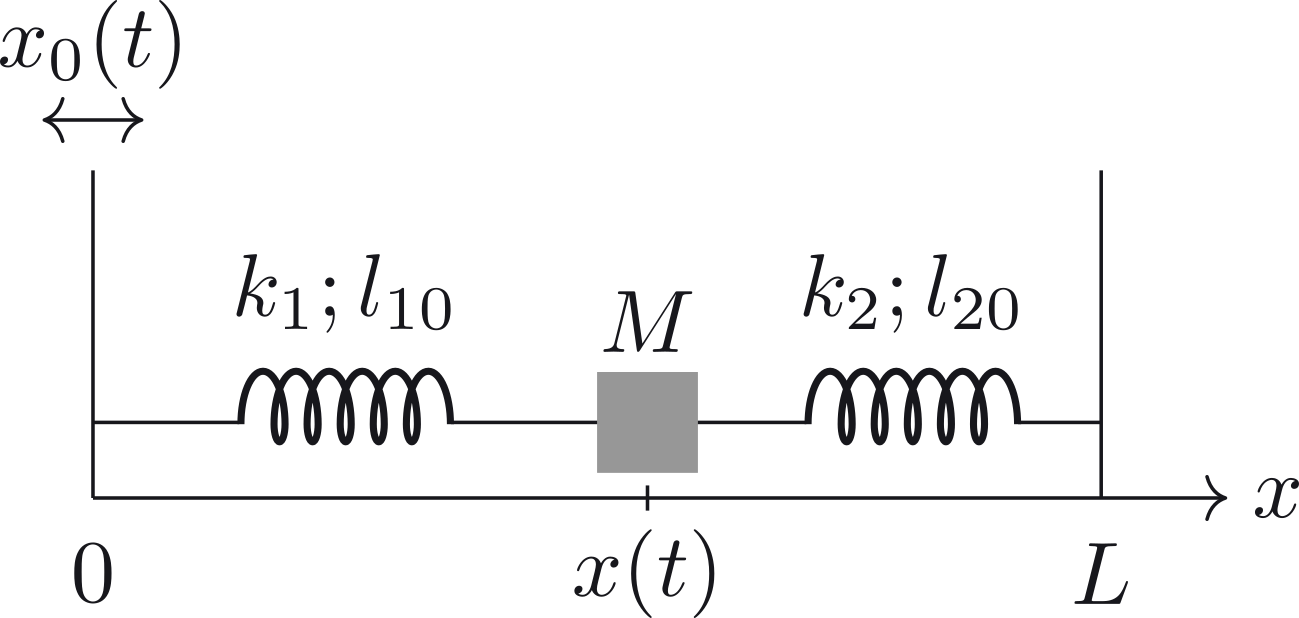
\includegraphics[width=\linewidth]{ressort-double_1}
		\end{center}
	\end{minipage}

	$M$ est relié à deux parois verticales par deux ressorts de raideurs $k_1$
	et $k_2$, de longueurs à vide $\ell_{10}$ et $\ell_{20}$. Celle de droite est
	immobile en $x = L$, celle de gauche, d'abscisse $x_0 (t)$, est animée d'un
	mouvement d'équation horaire $x_0 (t) = X_{0m} \cos(\wt)$. On supposera
	que $L = \ell_{10} + \ell_{20}$.
}

\QR{%
	Identifier les différentes forces s'exerçant sur $M$.
}{%
	~
	\smallbreak
	\vspace{-18pt}
	\begin{minipage}{0.43\linewidth}
		\begin{itemize}
			\item[b]{Système} : masse~;
			\item[b]{Référentiel} : $\Rc_{\rm sol} (O,x,y,t)$~;
			\item[b]{Position de la masse} : $\OM = x\ux$~;
			\item[b]{Longueur ressort 1} : $x(t) - x_0(t)$~;
			\item[b]{Longueur ressort 2} : $L-x(t)$.
		\end{itemize}
	\end{minipage}
	\hfill
	\begin{minipage}{0.57\linewidth}
		\textbf{Bilan des forces}~:
		\begin{enumerate}
			\item Poids $\Pf = -mg\uy$~;
			\item Réaction du support $\vv{R} = R\uy$~;
			\item Rappel du ressort 1
			      $\vv*{F}{1} = -k_1(\ell_1 - \ell_{10})\ux$~;
			\item Rappel du ressort 2
			      $\vv*{F}{2} = k_2(\ell_2 - \ell_{20})\ux$~;
			\item Force de frottement fluide $\vv{f} = -h\vf =
				      -h\dot{x}\ux$.
		\end{enumerate}
	\end{minipage}
}

\QR{%
	Déterminer la position d'équilibre $x\ind{eq}$ de $M$ lorsque la paroi
	de gauche est immobile en $x = 0$.
}{%
	Avec le PFD, on trouve
	\begin{gather*}
		m\af = \Pf + \vv{R} + \Ff_{1} + \Ff_{2} + \vv{f}\\
		\Leftrightarrow m\left(
		\begin{array}{c}
				\DS\dv[2]{x}{t} \\
				0
			\end{array}
		\right)
		=
		\left(
		\begin{array}{c}
				-k_1(\ell_1 - \ell_{10}) +k_2(\ell_2 - \ell_{20}) -h v \\
				-mg + R
			\end{array}
		\right)
	\end{gather*}
	La projection sur $\uy$ montre que la réaction du support compense le poids.
	Sur l'axe $\ux$ on trouve
	\begin{gather*}
		\boxed{m \dv[2]{x}{t} + h \dv{x}{t}
			= -k_1(\ell_1 - \ell_{10}) +k_2(\ell_2 - \ell_{20})}
	\end{gather*}
	En développant les longueurs comme indiqué question 1, on a
	\begin{gather*}
		\boxed{m \dv[2]{x}{t} + h \dv{x}{t} =
			-k_1(x(t) -x_0(t) -\ell_{10}) + k_2(L - x(t) - \ell_{20})}
	\end{gather*}
	À l'équilibre les dérivées de $x$ sont nulles, d'où
	\begin{gather*}
		0 = -k_1(x(t) - x_0(t) - \ell_{10}) + k_2(L-x(t) -\ell_{20})
	\end{gather*}
	Ainsi, avec $x_{0, \equ}(t) = 0$ et $L = \ell_{10}+\ell_{20}$ (d'après
	l'énoncé) puis $x(t) = x\ind{eq}$ (par définition), on a
	\begin{gather*}
		0 = -k_1(x\ind{eq} -0 - \ell_{10}) + k_2(\ell_{10} +
		\cancel{\ell_{20}} -x\ind{eq} -\cancel{\ell_{20}})\\
		\Leftrightarrow
		(k_1+k_2)(\ell_{10} - x\ind{eq}) = 0
	\end{gather*}
	Comme $k_1+k_2 > 0$, on trouve
	\[\boxed{x\ind{eq} = \ell_{10}}\]
}

\QR{%
	On introduit $X = x - x\ind{eq}$. Établir l'équation différentielle
	vérifiée par $X$ lorsque la paroi bouge.
}{%
	Cette fois-ci, on garde $x_0(t)$ dans l'équation. Il vient alors
	\begin{gather*}
		m\ddot{x} + h\dot{x} + (k_1+k_2)(x-x\ind{eq})  = k_1x_0(t)
	\end{gather*}
	et en effectuant le changement de variable $X = x-x\ind{eq}$, on trouve
	l'équation habituelle
	\begin{gather*}
		\boxed{m \ddot{X} + h \dot{X} + kX = KX_{0m}\cos(\wt)}
	\end{gather*}
	avec $k = k_1+k_2$.
}

\enonce{%
	Pour étudier le régime sinusoïdal forcé, on introduit les grandeurs
	complexes $\xul{x}_0(t) = X_{0m} \exp(\jwt)$, $X(t) = X_m \exp(\jj(\wt +
			\f))$ et $v(t) = V_m \exp(\jj(\wt + \phi))$ associées à $x_0(t)$, $X(t)$ et
	$v(t) = \dot X(t)$.
}

\QR{%
	Définir les amplitudes complexes $\xul{X}_0$, $\xul{X}$ et $\xul{V}$ de
	$x_0(t)$, $X(t)$ et $v(t)$.
}{%
	On a simplement $\Xu_0 = X_{0m}$, $\Xu = X_m\exr^{\jj\F}$ et $\Vu =
		V_m\exr^{\jj\F}$.
}

\QR{%
	En exprimant $\w_0$, $Q$ et $\alpha$ en fonction des données du
	problème, établir la relation~: \[\xul{V} = \dfrac{\alpha}{1 +
			\jj Q\left(\dfrac{\w}{\w_0} - \dfrac{\w_0}{\w}\right)} \xul{X}_0\]
}{%
	En utilisant l'équation différentielle mais en complexes et sous forme
	canonique, on trouve
	\begin{gather*}
		(\jw)^2\Xu + \jw \frac{h}{m}\Xu + \frac{k}{m}\Xu = \frac{k_1}{m}X_{0m}
		\Leftrightarrow
		\Xu =
		\frac{k_1X_{0m}}{m}\times
		\frac{1}{\dfrac{k}{m} - \w^2 + \jw \dfrac{h}{m}}
	\end{gather*}
	Étant donné que $V = \dv{X}{t}$, $\Vu = \jw\Xu$, soit
	\begin{align*}
		\Vu & =
		\frac{k_1X_{0m}}{m}\times
		\frac{\jw}{\dfrac{k}{m} - \w^2+\jw\dfrac{h}{m}}
		\\
		\Leftrightarrow
		\Vu & =
		\frac{k_1X_{0m}}{m}\times
		\frac{1}{\dfrac{h}{m} -\jj \dfrac{k}{m\w} + \jw}
		\\
		\Leftrightarrow
		\Vu & =
		\frac{k_1}{h - \jj \dfrac{k}{\w} + \jj m\w}X_{0m}
		\\
		\Leftrightarrow
		\Vu & =
		\frac{k_1/h}{1 + \jj \left( \dfrac{m\w}{h} - \dfrac{k}{h\w}
			\right)}\Xu_0
	\end{align*}
	Avec $Q\w_0 = \frac{k}{h}$ et $\frac{Q}{\w_0} = \frac{m}{h}$, on trouve
	bien
	\begin{gather*}
		\boxed{
			\Vu = \frac{\alpha}{1+\jj Q \left( \dfrac{\w}{\w_0} -
				\dfrac{\w_0}{\w} \right)}\Xu_0
		}
		\qavec
		\boxed{
			\left\{
			\begin{array}{rcl}
				\alpha & = & \dfrac{k_1}{h}       \\
				\w_0   & = & \sqrt{\dfrac{k}{m}}  \\
				Q      & = & \dfrac{\sqrt{km}}{h}
			\end{array}
			\right.
		}
	\end{gather*}
}

\QR{%
	Mettre en évidence l'existence d'une résonance de vitesse.
}{%
	L'amplitude réelle de la vitesse donne
	\begin{gather*}
		V_m(\w) = \frac{\alpha}{\sqrt{1 + Q^2 \left( \dfrac{\w}{\w_0} -
				\dfrac{\w_0}{\w} \right)^2}}X_{0m}
	\end{gather*}
	qui est maximale pour $\w = \w_0$. On observe donc bien une résonance en
	vitesse pour cette pulsation, avec $V_{\max} = \alpha X_{0m}$.
}
\end{document}
